\section{Single player flowchart and explanation~\ref{fig:singleplayer}}

\begin{figure}
    \centering 
    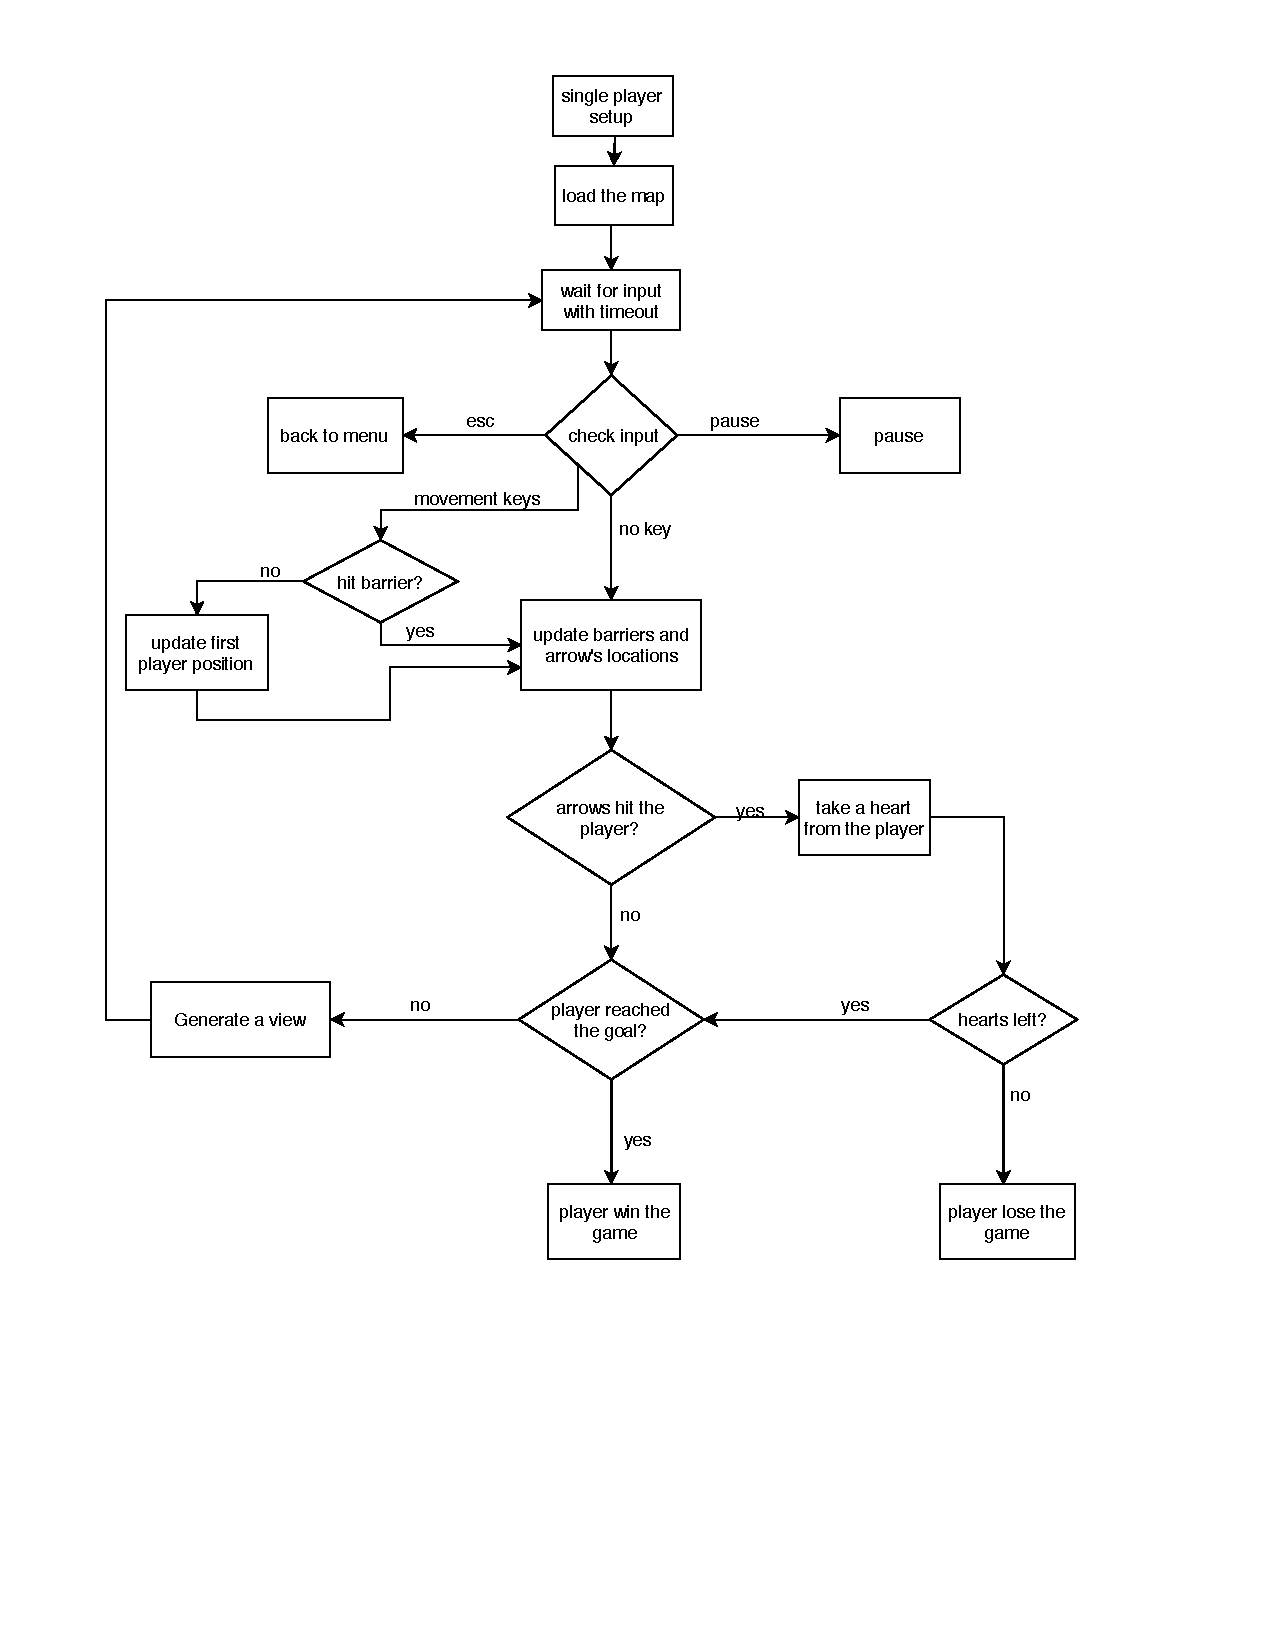
\includegraphics[width=\columnwidth]{singleplayer.pdf}
    \caption{Single player block flowchart }
    \label{fig:singleplayer}
\end{figure}

This flow chart explains all the steps happening on single player mode. 
As it is shown in Figure~\ref{fig:singleplayer}, load the map block reads the map from a text file. Next, we do some setups for single player game based on the map. In these setups we define a map with position of the player, the goal, the barriers and the arrows.
We should then read the input keyboard buffer and wait for input. The reading process is done within a limited time and there exist a timeout which expires if no input is provided within that time. Then the program checks the input to see what key has entered. If pause button is entered, program goes to pause game state. If escape button is pressed, program goes to menu. If no keys has entered, program updates the position of barriers and arrows as they are moving objects. If entered keys are movement keys, program first check if the player's move is permitted or not (checks map walls and barriers); if yes, then program updates the player position, barriers and arrows locations, and checks if the player is hit. If player can not move, program only updates barriers and arrows and does not change player's location. If player is hit by an arrow, it loses one heart and immediately checks if there is any heart left for the player. If the player loses all of its hearts, player loses the game. If the player has still a heart, program check if the player reaches the goal. Player wins the game if it reach the goal, otherwise program \textcolor{blue}{\bf generate a view} to display any updates on the map. Then wait for input key and it will continue until the player wins or loses the game.
If there exist any graphic related procedures it is done in generate view process, and logic of the game does not need to worry about graphics.

\subsection{Single player functions prototypes}
In this section we define the required functions prototypes and its relation to flow chart~\ref{fig:singleplayer}. We define some functions and the rest of the code will be in a main function. Comments above each function mention the associated block, the release, and assignee.

\begin{minted}{c}
#define MAP_MAX_NUM_OF_BARRIERS 10
#define MAP_MAX_NUM_OF_ARROWS 20
#define MAX_NAME_SIZE 100

typedef struct Position {
	int x;
	int y;
} Position;

typedef enum {
	DIRECTION_RIGHT,
	DIRECTION_LEFT,
	DIRECTION_UP,
	DIRECTION_DOWN
} Direction;

typedef enum {
	SPEED_LOW,
	SPEED_NORMAL,
	SPEED_HIGH,
} Speed;

typedef struct MapSpace {
	int xMin;
	int xMax;
	int yMin;
	int yMax;
} MapSpace;

typedef struct MapBarrier {
	Position currentPos;
	int length;
	Direction currectDir;
} MapBarrier;

typedef struct MapArrow {
	Position currentPos;
	Speed speed;
} MapArrow;

typedef struct Player {
    char name[MAX_NAME_SIZE];
	Position currentPos;
	int heart;
} Player;

typedef struct Goal {
	Position goal;
} Goal;

typedef struct Map {
	MapSpace space;
	int numberOfBarriers;
	int numberOfArrows;
	MapBarrier barrier[MAP_MAX_NUM_OF_BARRIERS];
	MapArrow arrow[MAP_MAX_NUM_OF_ARROWS];
	Goal goal;
	Player player;
} Map;

/* Block: Load the map - first release
 * Assigned to:
 * Load map information from an input file using provided information
 * from options.
 * Input: file_p
 * Output: Map */
Map loadMap(FILE* file_p);

/* Block: Update barriers and arrow's locations - first release
 * Assigned to:
 * Update barrier position in the map
 * Input: barrier, space
 * Output: barrier 
 * Return: void */
void updateBarrier(MapBarrier* barrier, MapSpace space);

/* Block: Update barriers and arrow's locations - first release
 * Assigned to:
 * Update arrows' position in the map
 * Input: arrow, space
 * Output: arrow
 * Return: void */
void updateArrow(MapArrow* arrow, MapSpace space);

/* Block: Pause - first release
 * Assigned to:
 * It continues the game when the game is on pause 
 * Input: void
 * Return: void */
void continueGame(void);

/* Block: Pause - first release
 * Assigned to:
 * It pause the game
 * Input: void
 * Return: void */
void pauseGame(void);

/* Block: Back to menu - first release
 * Assigned to:
 * It goes back to Menu
 * Input: void
 * Return: void */
void backToMenu(void);

/* Block: Hit barrier? - first release
 * Assigned to:
 * Check if there is any barrier on the way of player.
 * Input: player, barrier
 * Output: 0 ---> player no hit & 1---> player is hit
 * Return: int */
int isBarrierHit(Player player, MapBarrier* barrier_p, MapSpace space);

/* Block: Update player position - first release
 * Assigned to:
 * Update player position in the map.
 * Input: player, arrowKey
 * Output: player 
 * Return: void */
void updatePlayerPos(Player* player_p, int arrowKey);

/* Block: Arrows hit the player - first release
 * Assigned to:
 * check if the player is hit by arrows.
 * Input: player, arrow
 * Output: 1 ---> if the player is hit
 * Return: int */
int isPlayerHit(Player player, MapArrow* arrow_p);


/* Block: Takes a heart from the player - first release
 * Assigned to:
 * Takes a heart from the player.
 * Input: player
 * Output: player
 * Return: void */
void takeHeart(Player* player_p);

/* Block: hearts left - first release
 * Assigned to:
 * Check if the player lost all its heart.
 * Input: player
 * Output: 1 ---> if the player lost all its heart
 * Return: int */
int isGameOver(Player player);

/* Block: player lose the game - first release
 * Assigned to:
 * inform player that he/she lost the game
 * Input: player
 * Output: void
 * Return: void*/
void gameOver(Player player);


/* Block: player reached the goal - first release
 * Assigned to:
 * Checks if the player reached the goal
 * Input: player, goal
 * Output: 1 ---> if the player reached the goal
 * Return: int */
int isReachGoal(Player player, Goal goal);

/* Block: player win the game - first release
 * Assigned to:
 * inform player that he/she win the game
 * Input: player
 * Output: void
 * Return: void*/
void winGame(Player player);

/* Block: generate a view- first release
 * Assigned to:
 * Generate a 2d graphic map using updated information
 * Input: map
 * Return: void */
void updateView(Map map);

\end{minted}